\documentclass[11pt]{article}
\usepackage[T1]{fontenc}
\usepackage[utf8]{inputenc}
\usepackage{amsmath,amssymb,amsthm,booktabs,longtable,array}
\usepackage[margin=1in]{geometry}
\usepackage{hyperref,xurl}
\usepackage{tikz}
\newtheorem{theorem}{Theorem}[section]
\newtheorem{lemma}[theorem]{Lemma}
\newtheorem{proposition}[theorem]{Proposition}
\newtheorem{certificate}[theorem]{Exact certificate}
\newcommand{\Q}{\mathbb Q}
\newcommand{\wt}{\operatorname{wt}}
\newcommand{\rk}{\operatorname{rk}}
\newcommand{\HH}{\mathbb H}
\title{Compact arithmetic hyperbolic Coxeter polytopes:\linebreak
a dimension bound of 20}
\author{Coxeter Polytopes Frontier Project}
\date{20 October 2026; universal theorem manuscript}
\begin{document}
\maketitle
\begin{abstract}
We prove that compact arithmetic hyperbolic Coxeter polytopes have
dimension at most20. A companion dimension and field reduction leaves
only the actual ground field $\Q(\sqrt5)$ in dimension21.
The new ingredient is a normalized angle pool between distinct whole
components of the same spherical type. Its total vertex cost is one
nonnegative variable, while its local payments use actual component
multiplicities. Complete contact-star coverage and D5/H4 incidence
transfers permit an exact rational angle rule. Every
allowed finite rank 21 vertex forest has charge at most 40. Independently
evaluated native quadrilaterals have payment at least
$60007431727/60000000000>1$; the inherited triangle payment is at least 2.
A strict $h$-vector inequality forces average vertex charge greater than40,
a contradiction. With the earlier bound21 and the thirteen-field reduction,
this gives the dimension bound. The proof separates geometric coverage
of actual faces from the finite rational checks.
\end{abstract}

\section{Statement and scope}
A Coxeter polytope is a finite-sided convex hyperbolic polytope with facet
dihedral angles integral submultiples of $\pi$. Arithmeticity refers to
its reflection lattice and its actual Vinberg ground field. It is not a
condition on a convenient overfield containing displayed Gram entries.
\begin{theorem}\label{thm:main}
Every compact arithmetic hyperbolic Coxeter polytope has dimension at most 20.
\end{theorem}
The proof uses a preserved higher-dimensional reduction, the nongolden
field arguments below, and a golden-field step. We state the inherited
interfaces precisely so that their internal geometric proofs are not
confused with the published field restrictions.
\begin{proposition}[Companion dimension and field reductions]\label{prop:inherited}
Every compact arithmetic hyperbolic Coxeter polytope has dimension at
most21. If its dimension is21, its actual cyclic ground field is
$\Q(\sqrt5)$.
\end{proposition}
The first assertion is the dimension-specific composition through the
published compact ceiling29 in the preserved technical proof supplement
\path{manuscripts/compact_arithmetic21.tex}. The second uses the
dimension-at-least14 thirteen-field list and the twelve nongolden
dimension21 exclusions stated in Section~\ref{sec:fields}.
Their proof homes and exact interfaces are given there; neither
assertion is being imported as a published dimension20 theorem.
The rest of this paper excludes the remaining golden-field case.

Published inputs, internal geometric arguments, and finite exact checks
are distinct. Published assumptions include compact acute simplicity,
finite/affine and Lann\'er classification, the arithmetic cyclic-product
criterion and field restrictions, simplest-type reflection arithmeticity,
rational isotropy, and the nonnegative symmetric $h$-vector theorem
\cite{Vinberg,Nikulin,Belolipetsky}.
The supporting-star reduction, whole-component normalization, incidence
transfers and rational recurrence are internal proofs. Exact scripts
certify explicitly finite obligations; a numerical optimizer only
proposes a vector. The geometric completeness arguments precede the
finite evaluations.

\section{The strict counting threshold at rank 21}
A planar angle is an incidence $(v,F)$ of a vertex and a two-face. In
a simple $n$-polytope it corresponds to an unordered pair of incident
facet normals, marked in the finite vertex diagram.
\begin{lemma}\label{lem:threshold}
Suppose nonnegative planar-angle weights on a compact simple21-polytope
satisfy $\sum_{v\in F}\wt(v,F)\ge5-k$ on every $k$-gonal two-face.
Then the total vertex charge is at least $40f_0+550$, so its average
is strictly greater than40.
\end{lemma}
\begin{proof}
Each vertex is on $\binom{21}{2}=210$ two-faces. Double counting gives
\[
 \sum_v\wt(v)\ge5f_2-210f_0.
\]
For the symmetric nonnegative $h$-vector of the simplicial dual,
\[
 f_0=\sum_{i=0}^{21}h_i,\qquad
 f_2=\sum_{i=0}^{21}\binom{21-i}{2}h_i.
\]
Pair $i$ with $21-i$ for $0\le i\le10$. In $5f_2-210f_0$, their
coefficient on $h_i=h_{21-i}$ is
\[
 5\left[\binom i2+\binom{21-i}{2}\right]-420
 =80+5(i-10)(i-11)\ge80.
\]
The constant80 is their coefficient in $40f_0$. Every extra term is
nonnegative, and $i=0$ contributes $5\cdot10\cdot11\,h_0=550$ because
$h_0=1$. Hence $5f_2-210f_0\ge40f_0+550$.
\end{proof}
It suffices to pay2 on triangles and 1 on quadrilaterals; nonnegativity
handles $k\ge5$. An upper certificate equal to 40 is enough for a
contradiction. There is no need to manufacture a strict numerical margin.

\section{Complete supporting-star coverage}
We explain the geometric quantifiers needed for the new local weights.
Use the Lorentz form of signature $(21,1)$ and spacelike outward facet
normals $r_i$ with $(r_i,r_j)\le0$ for distinct walls. Chamber inequalities
are $(x,r_i)\le0$.
\begin{lemma}\label{lem:projection}
Every positive-definite principal root set defines an actual face. A
positive affine principal set is impossible in a compact chamber.
\end{lemma}
\begin{proof}
Let $B$ be the positive-definite principal Gram matrix and $h$ a strict
interior timelike vector. A positive-definite $Z$-matrix has entrywise
nonnegative inverse, so $c=B^{-1}((h,r_i))\le0$. The vector
$h_0=h-\sum_i c_i r_i$ is orthogonal to the chosen roots, has
\[
 h_0^2=h^2-((h,r_i))^TB^{-1}((h,r_i))<0,
\]
and has strictly negative product with every other facet normal. This
gives a relative-interior point of the face. For an affine principal set,
its positive kernel gives a nonzero null vector with nonpositive products
against every wall. It cannot be zero because pairing its positive
combination with $h$ is negative. It gives an ideal point, contradicting
compactness.
\end{proof}

Let $W$ be the 19 supporting roots of a quadrilateral and $b_0,b_1,b_2,b_3$
its cyclic side roots. Every adjacent extension of $W$ is elliptic.
Each opposite extension is indefinite by Lemma~\ref{lem:projection}:
otherwise the corresponding opposite sides would meet on this face.
Minimal indefinite subdiagrams contain both opposite black roots and
are Lann\'er pieces. Complete initial union supports retain shared white
roots, black identifications and every cross contact.

\begin{lemma}\label{lem:corank}
A $k$-root contact core containing a positive corner of order $k-2$ and a
negative direction has nullity at most one. A complete quadrilateral
star has nullity exactly one.
\end{lemma}
\begin{proof}
The positive index is at least $k-2$ and the negative index is one.
For the full star $k=23$ but the ambient Lorentz dimension is22, so it
is singular and the nullity is exactly one.
\end{proof}

\subsection{The finite seed and extension domains}

A contact state records the four cyclic side roots, the supporting
white roots already entered, all native labels, each fixed dotted
parameter, and the exact Gram data. Isomorphisms must preserve the
four marked roles and are accompanied by a checked diagonal gauge
congruence. A state is unpaid when no proved persistent part of the
baseline rule has already supplied a unit.

\begin{proposition}[Finite parameter domains]\label{prop:domains}
Every unpaid actual golden-field quadrilateral starts in one of the
opposite-pair union domains. At each state its next touching white
root belongs to a finite exact one-white domain. The dotted parameters
in the seed domains have finite integral bounds that remain valid in
every larger principal extension.
\end{proposition}
\begin{proof}
The finite-angle alphabet has no cutoff hypothesis. The two-cycle
$4\cos^2(\pi/m)=2+2\cos(2\pi/m)$ belongs to $\Q(\sqrt5)$;
its real cyclotomic degree is at most two. The candidates are
$2,3,4,5,6,8,10,12$, and $8,12$ generate the wrong quadratic
fields. Thus exactly $2,3,4,5,6,10$ remain.
For a three-node piece, enumerate the 56 unordered triples. Its
nonzero cycle belongs to the ground field precisely when the counts
of labels $4,6,10$ are even: the square classes of $2,3,\varphi+2$
are independent. Here $2,3,6$ are not squares in $\Q(\sqrt5)$,
and the norm of $\varphi+2$ is five. A right triangle has zero cycle
and needs no parity test. Exact physical determinant negativity and
conjugate determinant positivity leave the twelve listed triangle
types in the attached catalogue.
At order four or five, a bond at least six with a neighboring
nonright bond gives a proper three-node determinant at most
$1-3/4-1/4=0$; a dotted pair is already a nonpositive proper pair.
Thus the bonds are $3,4,5$. Any cycle must span all nodes and have
no chord: a shorter all-three cycle has a nonpositive all-ones
witness. Consequently enumerate all labeled trees (for example by
Pr\"ufer words), all spanning chordless cycles, and all assignments
$3,4,5$, then test every proper principal matrix, physical negative
index, field cycles and conjugate positivity. Quotienting only by
explicit label-preserving maps leaves six order-four and four
order-five records. An order-two dotted piece is retained symbolically
as $t\in\mathbb Z[\varphi]$, $t>4$, $0<t'<4$ until the bound below.
This defines the complete catalogue test used here; it does not
assert that a passing local diagram extends to a chamber.
The remaining radicands $2,3,\varphi+2$ are totally positive.
Once cycle products are fixed, alternative real radical signs differ
by diagonal root sign changes, so conjugate positivity is a well-defined
test independent of an arbitrary choice of displayed root signs.

For each opposite pair, a minimal indefinite subset contains both
black roots, since deleting either leaves a subset of an actual
finite corner. An affine principal subset is impossible by
Lemma~\ref{lem:projection}. The minimal pieces are therefore
Lann\'er diagrams of order at most five. Enumerate their allowed
white identifications and the remaining contacts in the union.
Every unfixed pair apart from the two opposite pairs belongs to an
actual finite corner. Its label belongs to the golden native
alphabet $2,3,4,5,6,10$; no dotted distance is sampled in filling
those pairs. Exact finite-corner and arithmetic tests give a finite
initial domain once the opposite dotted parameters have been bounded.

Here is the parameter bound used in the remaining24 minimal dotted
families. Their exact inertia certificates identify a common block
$B$, obtained by deleting the dotted endpoints0 and 2, that is
nonsingular and already has one negative direction. If the dotted
entry is $-x$ and the endpoint squares are $d_0,d_2$, its Schur
residual has the form
\[
 \begin{pmatrix}a&-x-c\\-x-c&b\end{pmatrix}.
\]
The residual must be positive semidefinite: the common block has
already used the permitted negative direction. Thus
\[
 (x+c)^2\le ab,\qquad
 t:=\frac{4x^2}{d_0d_2}\le\frac{8(ab+c^2)}{d_0d_2}.
\]
This is a principal-matrix obstruction and survives every extension.
The exact ceilings $U$ of the displayed upper bounds lie between9
and 76 in the finite family table. Cyclic integrality gives
$t=A+B\varphi\in\mathbb Z[\varphi]$, where
$\varphi=(1+\sqrt5)/2$. The physical and conjugate conditions give
\[
 4<t\le U,\qquad 0\le t'\le4.
\]
Hence $B=(t-t')/\sqrt5$ is positive and at most $U$. Also
$A=(\varphi t'-\varphi't)/\sqrt5$ lies between0 and $U$:
use $U\ge4$ and $\sqrt5-|\varphi'|=\varphi$ for the upper
bound. The integer box $0\le A\le U$, $0<B\le U$ is therefore
complete. Every point is tested for the exact field and gauge,
cycle integralities, physical inertia and conjugate positivity.
The recorded evaluation gives532 parameter candidates and 32
necessary surviving seeds. Passing these tests is not an assertion
of geometric realization.

Finally, an added white root belongs to all four actual finite
corners. Its products with entered roots are finite native labels
from the same alphabet. Enumerate all label tuples with at least
one nonright contact to the current core, retaining exactly those
whose four enlarged corners are finite and whose exact arithmetic,
root relations and embedding inertias pass the necessary tests.
Equivalently, generate the tuples by complete finite-Dynkin
attachment. The old dotted invariant stays fixed; a new supporting
white introduces no free dotted parameter. This proves finiteness
and the required coverage of a single extension.
\end{proof}

The finite Lann\'er family table, minimal-union enumeration and the
24 exact Schur bounds are internal certificate inputs. Their full
domains and independent checks are in
\path{results/fresh_sqrt5_quad_exhaustion_20261015.md} and
\path{results/fresh_sqrt5_dotted_parameters_20261015.md}.
The argument above explains why those finite tables suffice; checking
their hashes alone would not establish that reduction.
Here is the data interface used by those inputs. A diagram record has
its ordered nodes, the lexicographically ordered array of pair labels,
the four fixed black roles, and the white subset. Its exact Gram
normalization records the diagonal root squares and field entries;
any alternate labeling carries an explicit mark-preserving diagonal
gauge congruence. A dotted-family record additionally gives the deleted
endpoint indices, the exact matrix $B$, its inertia pivots, the Schur
entries $a,b,c,d_0,d_2$, and the integral ceiling $U$ proved by their
displayed inequality. All numbers are rational pairs in the integral
field basis or specified totally real radicals, not decimal eigenvalues.
The finite table is checked by exact proper-principal positivity,
physical negative index, cycle integrality and conjugate positivity.
The independent minimal-union replay uses finite-Dynkin recognition
and separate literal white-identification generation. These finite
classified tables are attached proof data, while the all-extension
coverage argument is Proposition~\ref{prop:coverage} below.

\subsection{The contact queue and its stopping obligations}

The algorithm begins with every retained marked seed and preserves
its literal seed map. Process each new representative once. Record
every singular state as a stopping obligation, including a singular
state that also has accepted children. Otherwise generate the entire
one-white domain of Proposition~\ref{prop:domains}. A branch may be
discharged by a uniform proof of persistent payment, rejected by a
necessary-condition failure, or retained with its exact marked child
map. A conditionally sealed unpaid state permits only orthogonal
spectators. At31 roots retain a singular obligation and reject a
nonsingular core by rank.

\begin{proposition}[Termination]\label{prop:queue-termination}
The contact queue is finite, independently of a time or memory limit.
\end{proposition}
\begin{proof}
A $k$-root core has a positive corner of order $k-2$ and a negative
direction, so its rank is at least $k-1$. The published compact
ceiling29 allows ambient Lorentz rank at most 30. Thus at most 31
roots can occur; at31 only a singular core can remain. There are
finitely many seed parameters, finitely many native label tuples
at each extension, and a uniform bound on the number of extensions.
Consequently even the labeled state tree is finite. Passing to
representatives by verified marked isomorphisms preserves this
property. Each representative is processed once, so the algorithm
halts. Its completeness still requires the actual-face argument below.
\end{proof}

\begin{proposition}[Final touching-star principle]\label{prop:coverage}
For an unpaid actual quadrilateral, the inherited complete finite/dotted
contact queues contain a final contact representative whose marked
components are entire. Its remaining supporting components are common
orthogonal spectators. Singular states that can extend must also remain
stopping obligations.
\end{proposition}
\begin{proof}
Begin with the actual opposite-pair minimal union. In each white
component touching the entered core, order unentered vertices starting
with a contact to that core and continuing along connected white edges.
Every next root belongs to its complete one-white contact domain.
Rejected arithmetic, signature or conjugate profiles cannot occur.
A profile producing persistent basic payment pays the face independently
of all adjustable bonuses. Otherwise a literal retained child map applies.

At a conditionally sealed state any further touching contact would give
such persistent payment; hence the unpaid actual face has only orthogonal
spectators. At an unsealed singular state continue while actual touching
roots remain. Choose the final such state, rather than an earlier
embedded singular subcore. Its contact part has corank one after the
positive spectator block is split off, by Lemma~\ref{lem:corank}. It has
at most 23 roots. The complete queues retain every singular stopping
state, including expandable and boundary states, within their larger
geometric root bound. Its marked components are therefore whole in the
actual corners. The remaining components are orthogonal to the black
and entered white roots.
\end{proof}
Propositions~\ref{prop:domains}--\ref{prop:coverage} separate three
obligations: finite extension domains, termination, and geometric
coverage by final representatives. The recorded finite queue has5172
states and 51599 contact profiles; its2070 singular obligations include
expandable states. The dotted queue has438 states,5146 profiles and 264
singular obligations. All423 dotted states below31 roots have complete
extension domains. These are computed outputs of the stated algorithm.
The exact maps and the independent queue evaluations are documented in
\path{results/fresh_sqrt5_nonsingular_rank29_fast_20261015_review.md}
and \path{results/fresh_sqrt5_dotted_rank29_exhaustion_20261015_review.md}.
The final rational evaluator reads this saved domain; it does not
regenerate either queue.

The rank 21 native iterator combines the prior complete parameter-stress
inventory with every fitting singular finite-queue state. There are1979
native faces. For an $N$-root contact row, common spectator rank is
$23-N$. Enumerate exact external counts $(e,f,g,j)$ of
$A_1,I_2(5),H_3,A_4$ with
\[
 e+2f+3g+4j\le23-N,\qquad
 23-N-e-2f-3g-4j\ne1.
\]
There is no untracked rank-one type; $A_2,A_3$ realize every residual
rank at least two. The same spectator forest is used at all four
corners. This gives102917 cases. Exact component multiplicities determine
all denominators. A numerical payment from an embedded old subcore is
not substituted for the actual new angle.

\section{The angle rule and its geometric exceptions}
Write $q=(a,b,h,d)$ for the exact numbers of entire
$A_1,I_2(5),H_3,A_4$ components. Old coefficients use the capped selector
$c=(a,\min(b,2),\min(h,1),\min(d,2))$.
The fixed baseline on a whole connected component $C$ is
\[
 B(C;i,j)=\mathbf1_{\operatorname{dist}_C(i,j)\le2}
 +\mathbf1_{C=H_4}\mathbf1_{\{\operatorname{dist}_C(i,j)=3\}
                      \text{ or }\{ij\text{ is the five-edge}\}}.
\]
\begin{lemma}[The baseline triangle payment]\label{lem:triangles}
Every triangular two-face has baseline payment at least two, including
arbitrary additional supporting roots.
\end{lemma}
\begin{proof}
A minimal indefinite principal subset of its star contains all three
black roots: omitting any one leaves an actual positive corner.
Compactness excludes an affine principal subset. The complete golden
Lann\'er table therefore gives
$12+6\binom43+4\binom53=76$ three-black markings.
The exact finite check takes each catalogue graph, each black triple,
and each omitted black root, and computes the distance and entire
$H_4$ bonuses in the remaining positive graph. Sixty-nine markings
already have distance-two total at least two. Here is the entire
deficient list, with numbered vertices $0,\ldots,4$; unlisted bonds
are right. Corner triples are in increasing order of the omitted black.
\[
\begin{array}{c|c|c}
\text{nonright edges}&\text{black triple}&\text{baseline corner weights}\\ \hline
04=14=34=3,\ 23=5&012&(1,1,1)\\
04=13=14=3,\ 23=5&023;024&(2,0,0);(1,1,0)\\
04=4,\ 13=14=3,\ 23=5&023;024&(2,0,0);(1,1,0)\\
04=23=5,\ 13=14=3&023;024&(2,1,0);(1,2,0).
\end{array}
\]
The catalogue and these literal markings, not sampled wall distances,
are the finite data checked in the triangle certificate.
Every path already present remains the unique path in a finite
spherical extension, so its distance cannot increase. A finite
component containing an induced $H_4$ is that whole $H_4$, by the
finite classification of diagrams with a $5$ bond. Thus each extra
unit used in the table survives every additional white root.
Disconnected marked nodes can only gain a nonnegative payment.
This proves the full-star assertion. No extra $I_2(5)$ or $H_3$
five-edge payment is needed for this lemma.
\end{proof}

We now define every coefficient orbit of the additional rule. A rooted
type means a finite labeled connected diagram with one distinguished
node, modulo label-preserving isomorphism; a pair type has an unordered
distinguished node pair. The data give a nonnegative rational value
$v_c(\mathfrak o)$ for each orbit and capped context $c$; unlisted
values are zero. For an actual marked angle use this exhaustive,
mutually exclusive selector:
\begin{enumerate}
\item If both marks lie in one component, add its pair-type value
only when its baseline is zero. There is no multiplicity denominator.
\item Otherwise order the first three hub families as
$A_1<I_2(5)<H_3$. If one marked component is a hub and the other is
not in that family or any earlier hub family, use the first such hub
$H$ as source. The orbit records $H$, the destination family and its
rooted type, and the addition is $v_c(\mathfrak o)/(\rk(H)k_H)$,
where $k_H$ is the exact number of whole $H$ components. It is
independent of the selected source root. Thus the denominators are
$a,2b,3h$, and an $A_1$--$H_3$ angle, for example, belongs only
to the $A_1$ source family.
\item If no preceding selector applies and both components are
$A_4$, use their unordered pair of rooted types and divide its value
by $4(d-1)$; this branch exists only for $d\ge2$.
\item If exactly one component is $A_4$ and the other is none of the
four hub types, the orbit records both rooted types, with $A_4$ first,
and the addition is its value divided by $4d$.
\item All remaining cross-component angles have no old bonus.
\end{enumerate}
This defines a literal angle from its whole finite vertex diagram and
the attached rational coefficient table, without calling an optimizer.
Rooted and pair orbits can be encoded recursively by the labeled tree
rooted at its center, recording at each node its mark and the sorted
list of labeled child codes; two-center trees use the unordered two
halves and their joining label. The attached variable-order table
identifies these codes and contexts. Numeric column indices are merely
serialization, not part of the mathematical rule.

At fixed $c$ these old charges are additive over components.
For each destination root, summing a hub source over all $\rk(H)k_H$
source roots cancels its denominator. An $A_4$ source similarly
contributes one fourth of the sum over its four rooted types to each
destination root. For distinct $A_4$ factors, summing over factor
pairs gives
$\binom d2[4(d-1)]^{-1}\sum_{s,t\in A_4}v_c(\{s,t\})
=(d/8)\sum_{s,t\in A_4}v_c(\{s,t\})$.
These identities define the additive type costs $w_c(T)$ used below.

\subsection{D5 and H4 incidence transfers}
These internal geometric lemmas are used with their complete written
proofs and exact coefficient certificates.
\begin{proposition}[Previously proved priority rules]\label{prop:priority}
Let $W$ denote the old total charge and $b$ the old extreme-$E_8$ pair
bonus. There is a nonnegative angle rule preserving all required
small-face payments with the following conservative allowances:
\begin{center}
\begin{tabular}{ll}\toprule
Whole vertex forest&Allowance\\\midrule
$D_5+2E_8$&$W-\min(1,2b)$\\
$A_1+H_4+2E_8$&$W-t$\\
$A_1+A_4+2E_8$, $A_5+2E_8$&$W+t$\\
$A_1+B_4+2E_8$, $B_5+2E_8$&$W+t$\\
All other forests&$W$\\\bottomrule
\end{tabular}
\end{center}
Here $0\le t\le1$. The two D5 state inequalities must both be imposed.
\end{proposition}
We prove both priority rules, including their simultaneous consumers.
All roots in the local calculations below have square two unless a
label-four scaling is specified. Put $s=\sqrt5$, $\varphi=(1+s)/2$
and $\mathcal O=\mathbb Z[\varphi]$. A whole untouched $E_8$ is
orthogonal to any new side seen in a finite corner: it has no connected
finite extension. Thus its roots really split off in each calculation.

\subsubsection{The triangle activity and the D5 fork deletion}
Number $D_5$ by edges $01,12,23,24$, with short leaves $A=3,B=4$.
The complete necessary nonadjacent triangle domain has the following
third-wall contacts; all unspecified products are zero:
\[
\begin{array}{c|c|c}
\text{old type}&\text{contact magnitudes}&\text{marked triangles}\\ \hline
D_5&\varphi@0&(0,2)\\
D_5&\varphi@f\text{ or }1@1+\varphi@f,\ f=3,4&(1,f)\\
E_8&\varphi@0&(0,2)\\
E_8&\varphi@6&(3,5),(3,6),(4,6).
\end{array}
\]
Here $E_8$ is the path $0-1-\cdots-6$ with $7$ attached at $2$.
For clarity, this is a finite exact domain calculation: for each
nonadjacent marked pair generate every finite one-node extension of
the corner with one mark deleted, then give the other mark each
contact $2,3,4,5$ and test the other corner. A bond at least six to
any old node would have to be an isolated $I_2(m)$ in every corner,
impossible because an old neighbor remains. Test positive physical
height $H=g^TJ^{-1}g-2$, cycle membership in $\mathbb Q(s)$,
conjugate $H'\le0$, and all affine principal subsets. These literal
finite tests leave exactly the displayed list; the complete eligible
vectors and exact tests are supplied with the triangle-domain data.
No high-label cutoff or geometric realizability filter is imposed.
The $D_5$ fork pair is absent, so it is never triangular.
The two $E_8$ root heights are $4+2s$ and $1+s$.
Let $I_E$ indicate the occurrence of any of these four triangles in
either whole $E_8$; there are eight designated possible triangles.

Consider a fork quadrilateral with cyclic sides $A,B,c,d$ and white
$W=\{0,1,2\}$. If it has a basic unit not being deleted, it is paid.
Otherwise $c\cdot d=0$, and finite extension of the endpoint $A_4$
permits precisely
\[
 N,\quad P_{03},P_{04},P_{13},P_{23},
\]
where $N$ is no contact and $P_{ij}$ is contact at white $i$ with
label $j$. A contact to the adjacent old black root would already
be a retained adjacent-pair unit. A rank-five finite extension of
$A_4$ is $A_5,B_5,D_5$, so there are no other endpoints or high bonds.
Testing $W+c+d$ as a finite tree leaves exactly the eleven unordered
pairs in the next table. All excluded pairs have a cycle, degree-four
vertex, or a branched finite diagram with an internal four-bond.

The all-distance arithmetic reduction is short enough to give
explicitly. A label-three side can be field-scaled to square two
and contact $-1$; its old three-path cycle makes its opposite
product an element of $\mathcal O$. A label-four side is instead
scaled to square four and contact $-2$; the Cartan cycle still
makes its opposite product integral, with no lost factor of two.
In that cycle the two incident factors are $-2$ and $x/2$;
the old label-three path contributes signs only, leaving $\pm x$.
For an $N$ side use the invariant opposite square $X\in\mathcal O$,
without assuming its norm-two root field-valued. The complete finite
opposite lists, subject to the strict opposite-corner inequalities,
are
\[
 x=-2\cos(\pi/m)\in\mathbb Q(s):\quad-1,-\varphi;
 \qquad X>5/2:\quad\varphi^2,3,(5+s)/2.
\]
A square-four side has only the finite field-valued opposite value
$-2$. Indeed the two-cycle restricts the labels to $2,3,4,5,6,10$;
other values require $\sqrt2,\sqrt6$ or $\sqrt{5+s}\notin\mathbb Q(s)$.
The same cyclotomic restriction follows from degree at most two of
$4\cos^2(\pi/m)$, so it is not a sampled list.

Eliminating $W$ uses
$J_W^{-1}=\frac14\left(\begin{smallmatrix}3&2&1\\2&4&2\\1&2&3\end{smallmatrix}\right)$.
For the following notation let
\[
\begin{split}
 f_0(X,y)&=(5-2X)(3+y-2y^2)+3y-7,\\
 f_1(X,y)&=(5-2X)(1+y-y^2)+3y-5,\\
 f_2(x,y)&=(2x-3)((x+1)y^2-(x+2)y)-2(x-1)^2,\\
 f_3(x,y)&=(2y+1)(3+x-2x^2)+3x-7,\\
 f_4(x,y)&=(2y+1)(1+x-x^2)+3x-5.
\end{split}
\]
Corank one gives exactly these equations and the three unit equations:
\begin{center}\small
\begin{tabular}{lll}\toprule
Endpoints&corank equation&disposition\\ \midrule
$N,N$&$(2X-5)(2Y-5)=9$&Lambert branch below\\
$N,P_{03}$&$f_0(X,y)=0$&excluded\\
$N,P_{04}$&$f_1(X,y)=0$; square-four $y$&excluded\\
$N,P_{13}$&$f_1(X,y)=0$&excluded\\
$P_{03},P_{13}$&$f_2(x,y)=0$&excluded\\
$N,P_{23}$&$(5-2X)(2y+1)=9$&unit branch below\\
$P_{03},P_{23}$&$f_3(x,y)=0$&excluded\\
$P_{04},P_{23}$&$f_4(x,y)=0$; square-four $x$&excluded\\
$P_{23},P_{23}$&$(2x+1)(2y+1)=9$&excluded\\
$P_{03},P_{03}$&$(x+1)(y+1)=1$&unit branch below\\
$P_{13},P_{23}$&$f_4(y,x)=0$&excluded.\\ \bottomrule
\end{tabular}\end{center}
These are exact Schur determinants, not assumptions about opposite
lengths. Each excluded row forces at least one opposite pair finite.
For $f_0$, solving for $X$ gives
$X-4=(3y^2-8)/(3+y-2y^2)<0$ if $y\le-2$.
For $f_1$ the denominator is $2(1+y-y^2)$ with the same numerator.
For $f_3,f_4$, solving for $y$ gives
$y+2=(8-3x^2)/(3+x-2x^2)$ or
$(8-3x^2)/(2(1+x-x^2))>0$ in the dotted range.
For $f_2$ at $x,y\le-2$, its left side is at least
$f_2(x,-2)=2(5x^2+x-13)\ge10$.
Thus there is no unbounded opposite-distance search.
Substitution of the complete finite lists gives all the obstructions:
\begin{center}\small
\begin{tabular}{lp{.72\linewidth}}\toprule
Row&nonintegral value or nonsquare discriminant\\ \midrule
$N,P_{03}$&$y=-\varphi$ gives $X=(25+12\varphi)/11$;
finite $X$ gives $134\pm50s,84$, norms $5456$ or rational nonsquares.\\
$N,P_{13}$&$y=-1,-\varphi$ gives $13/2,2+5\varphi/4$;
finite $X$ gives $26-6s,28,34+14s$, norms $496,784,176$;
$28$ is neither a rational square nor five times one.\\
$N,P_{04}$&finite square-four $y=-2$ gives $X=18/5$;
finite $X$ has the preceding discriminants.\\
$P_{03},P_{13}$&$x=-\varphi$ gives $73+89\varphi$ of norm $3905$;
$y=-1,-\varphi$ gives $104,153+224\varphi$, norm $7505$ for the latter.\\
$P_{03},P_{23}$&$x=-\varphi$ gives $y=-(3+12\varphi)/11$;
$y=-1,-\varphi$ gives discriminants $21,134+50s$, the latter of norm $5456$.\\
$P_{04},P_{23}$&$x=-2$ gives $y=-8/5$; $y=-1,-\varphi$
gives $28,34+14s$, the latter of norm $176$.\\
$P_{13},P_{23}$&finite $y=-1,-\varphi$ gives $x=-9/2,-5\varphi/4$;
finite $x=-1,-\varphi$ gives $28,34+14s$.\\ \bottomrule
\end{tabular}\end{center}
For a nonrational square in $\mathbb Q(s)$ its rational norm must
be a rational square; a rational number must be a square or five
times a square in $\mathbb Q$. These tests exclude every listed
branch. In the $P_{23},P_{23}$ row, both dotted implies $x=y=-2$,
whose rational indefinite Gram violates conjugate positivity.
Finite $x=-1$ gives $y=-5$, with rational opposite principal
 determinant $-21$; $x=-\varphi$ gives $y=-1/2-9s/10\notin\mathcal O$.
This also excludes its exchanged cases. In particular the mixed
$P_{13},P_{23}$ row is impossible: no fixed D5 half-units are being
silently added to the golden baseline.

Here are the complete unit branches. Every positive unit of
$\mathcal O$ is $\varphi^r$: scale it into $[1,\varphi)$ and use
its norm $\pm1$ and the fact that its conjugate difference is an
integer multiple of $s$. Norm $-1$ makes $r$ odd. Both $2$ and $3$
are inert, since $t^2-t-1$ has no root modulo either prime.
For $N,N$, set $U=2X-5,V=2Y-5$. Opposite indefiniteness and conjugate
positivity give
\[
 UV=9,\quad U,V>0,\quad -5\le U',V'\le-9/5,\quad U,V\equiv1\pmod2.
\]
\begingroup
\emergencystretch=1em
Thus $U=3^a\varphi^r$, $a=0,1,2$, $r\equiv3\pmod6$.
The conjugate interval leaves only $(a,r)=(0,-3),(2,3)$:
neighbors differ by a factor $\varphi^6>16$ and are already outside.
Hence $\{X,Y\}=\{\varphi^2,(23+9s)/2\}$.
For $N,P_{23}$ use $U=2X-5,V=-2y-1$ with the same conditions.
The two branches are
$(X,y)=(\varphi^2,-(19+9s)/2)$ and
$((23+9s)/2,(1-s)/2)$; the latter has a forbidden opposite product
in $(-1,0)$. In the former a side has just the short-leaf contact
$-\varphi$ at each of its two fork corners.
For $P_{03},P_{03}$ put $U=-x-1,V=-y-1$.
Now $UV=1$, $U,V>0$, and conjugate positivity gives
$-5/2\le U',V'\le-2/5$. Only $r=\pm1$ remains, so
$\{x,y\}=\{-\varphi,-\varphi^2\}$.
\par
\endgroup

These three surviving necessary patterns have no $E_8$ triangle
at any fork corner. For the first two, the short-leaf side height
is $H_L=(-1+5s)/8$; its length-two cyclic products with the two
$E_8$ triangle walls would be $(23+9s)/4$ and $3+s/2$, not in
$\mathcal O$. For the third, its side has height
$H=(1+9\varphi)/4$ and the corresponding products are
$(19+29\varphi)/2,(9+10\varphi)/2$, again nonintegral.
The other fork corner has identical contacts after white-path reversal.
Thus none of their fork units is deleted when $I_E=1$.
All eight other patterns were excluded. Every affected quadrilateral
therefore retains a full basic unit even when several active fork
units are removed. No triangle is altered, and on a longer face
removing one unit from its unit angle preserves nonnegativity.
This proves the active-state saving one on every $D_5+2E_8$ vertex.

\subsubsection{Inactive extreme-E8 consumers, with every D5 contact}
At the extreme pair $(0,6)$ of one old $E_8$, let
$W_E=\{1,2,3,4,5,7\}=D_6$; the whole old $D_5$ and second $E_8$
are white spectators. Suppose a quadrilateral has no other basic
unit. Its new walls are orthogonal. Deletion $0$ leaves $D_7$,
so the complete zero-payment endpoint types for $c$ are
$N$, $S=3@1$, $T=3@7$. Deletion $6$ leaves $E_7$, giving for
$d$ the types $N$ or $L=3@5$.
Any $S,T,L$ side is orthogonal to $D_5$: joining the old factors
would give an unlisted rank-thirteen finite tree with two forks.
An $N$ side may contact $D_5$ by long-leaf $3$ or short-leaf $3$,
with projection square $\delta=0,1,5/4$. If both do, only distinct
long/short attachments are finite, with mutual projection $C=1/2$.
This follows by finite D/E classification; two short attachments give
an affine $(2,2,2)$ tree, and repeated leaves give two forks.
Thus these statements include every spectator contact, not only a
previously selected orthogonal configuration.

The needed old inverse entries are
$J_{00}=4,J_{01}=7,J_{07}=5,J_{11}=14,J_{77}=8$,
$J_{55}=6,J_{56}=3,J_{66}=2,J_{06}=2$.
Eliminating $W_E$ gives old-black matrix
$\left(\begin{smallmatrix}1/2&-1/2\\-1/2&1\end{smallmatrix}\right)$.
For $N$ opposite squares $X,Y$, write $a=2-\delta_c,b=2-\delta_d$.
Conjugate positivity gives $0\le X'\le a/4$, $0\le Y'\le b/2$.
For the field-valued opposite products $\alpha$ of $S,T$ and
$\beta$ of $L$, it gives respectively
$\alpha'\in[3/2,2],[1,3/2]$, $\beta'\in[1,2]$;
these are the roots of the height polynomials
$12-14\alpha+4\alpha^2$, $6-10\alpha+4\alpha^2$,
$4-6\beta+2\beta^2$.

The corank equations are
\[
\begin{array}{c|l}
S,L&(\alpha-1)\beta=1\\
T,L&(1-2\alpha)(-\beta)=2\\
N,L&(2X-a)(-\beta)=a\\
S,N&(1-\alpha)(Y-b)=b/2\\
T,N&(1-2\alpha)(Y-b)=b.
\end{array}
\]
Every displayed unit factor is physically positive by opposite
indefiniteness. The unit proof above gives the following complete
short intervals (negative conjugates are essential):
\[
\begin{array}{c|c|l}
UV&U'\text{ interval}&U\\ \hline
1&[-1,-1/2]&\varphi\\
1&[-2,-1]&\varphi^{-1}\\
2&[-2,-1]&\varphi^{-1},2\varphi\\
3&[-3,-3/2]\text{ or }[-2,-1]&\varphi^{-1},3\varphi.
\end{array}
\]
They follow from $U=p^a\varphi^r$, $a=0,1$, $r$ odd; the adjacent
odd exponents already lie outside the interval. Applying them gives
all mixed-endpoint obstructions:
\[
\begin{array}{c|ccc}
&\delta=0&\delta=1&\delta=5/4\\ \hline
N,L&\beta=-\varphi^{-1}&X=\varphi^2/2\notin\mathcal O&
 8X-3=\varphi^{-1}\text{ or }3\varphi\\
S,N&\alpha=1-\varphi&2(1-\alpha)(Y-1)=1&
 (1-\alpha)(8Y-6)=3\\
T,N&1-2\alpha=\varphi^{-1}\text{ or }2\varphi&
 1-2\alpha=\varphi^{-1}<1&
 1-2\alpha=\varphi^{-1}\text{ or }3\varphi.
\end{array}
\]
Entries give either a forbidden finite product in $(-1,0)$, a
positive opposite product, a nonintegral coordinate, or the displayed
modulo-two contradiction. The $S,L$ row gives $1-\alpha=\varphi$,
again forbidden; $T,L$ gives the same positive/nonintegral alternatives
as its table row. Thus every pattern except $N,N$ is excluded.

For $N,N$ the complete equation is
\begin{equation}\label{eq:E8consumer}
4XY-4bX-2aY+ab-4C\sqrt{XY}-C^2=0,
\qquad X>a/2,\quad Y>b.
\end{equation}
With at most one $D_5$ contact, $C=0$ and it factors as
$(2X-a)(Y-b)=ab/2$.
The nonzero contact pairs $(\delta_c,\delta_d)=(1,0),(5/4,0)$
give respectively nonintegral $X=\varphi^2/2$ or
$8X-3=\varphi^{-1},3\varphi$.
The pairs $(0,1),(0,5/4)$ give respectively
$2(X-1)(Y-1)=1$ or $(X-1)(8Y-6)=3$, impossible modulo two.
For both contacts $C=1/2$ and the Cartan cycle gives
$t=\sqrt{XY}\in\mathcal O$.
The long/short orientation gives
$8t^2-4t+1-6X-4Y=0$, impossible modulo two.
The short/long orientation gives
$8t^2-4t+1-8X-3Y=0$.
Here $X'\le3/16$ excludes every finite $X$ from the two-cycle list;
if $X,Y\ge4$, the left side of \eqref{eq:E8consumer} is
$\ge69/2>0$. Hence $Y$ is finite, and $Y>1,Y'\le1/2$ leaves
only $Y=\varphi^2$. Substitution gives discriminant $20+8s$ of
norm $80$, not a square. This excludes the last $D_5$ contact.
For no contacts, $(X-1)(Y-2)=1$ and the short unit intervals give
$X=Y=\varphi^2$. Thus the two new sides are exactly the actual
$E_8$ triangle walls $F_0,F_6$ of the preceding table: their other
positive replacements close the designated triangle bundles.

Consequently, when $I_E=0$, an extreme-E8 quadrilateral must have
another basic unit. That unit cannot be an actively deleted $D_5$
fork unit: the old whole $D_5$ is white and cannot join the white
$D_6$ into a finite component with two forks. Its component after
adding the marks has rank at most seven, hence cannot turn into an
$E_8$ at another $D_5+2E_8$ corner. There it remains the whole white
$D_5$, so the black marks cannot be its fork leaves. This proves
simultaneous safety of inactive E8 deletions and active D5 deletions.
Inactivity also excludes triangles at that extreme pair; longer faces
need only nonnegative weights. Removing its nonnegative bonus is safe.
The two whole E8 copies have the same context and bonus $b$, so the
inactive saving is $2b$, while the active saving is one. Imposing
both physical-state rows gives exactly $W-\min(1,2b)$.

\subsubsection{The H4 deletion and all four source capacities}
Number $H_4$ as $0-1-2-3$ with bonds $5,3,3$, and its whole $A_1$
as node $4$. Remove $t$ from the extra five-edge unit at the target
$A_1+H_4+2E_8$. A triangular face at $(0,1)$ has third side $c$
orthogonal to both E8 factors. A contact label at least six to an
old nonisolated root is incompatible with its retained old neighbor,
except possibly at marked leaf $0$. That exception gives a retained
ordinary unit at the other triangle corner, and the old ordinary
five-edge unit gives the second. A high bond to the whole $A_1$
forces every H4 contact zero, giving height
$(2\cos(\pi/m))^2/2-2<0$. Thus every potentially deficient case
lies in the exact domain $\{2,3,4,5\}^5$.

The bounded test has no unspecified geometric filter. Let $g_i$
be the five contact magnitudes, $J=J_{H_4}\oplus(2)$ and
$H=g^TJ^{-1}g-2$. For all $4^5$ label vectors test both old-root
replacements by finite classification, $H>0$, field membership of
each old-path cycle, $H'\le0$, and all connected affine principals
containing $c$. Subsets containing a $5$ need no affine test, since
no affine Coxeter diagram has such a bond. There are 46 finite-corner
eligible vectors, four with nonpositive height, eight failing cycle
membership, and 34 remaining necessary vectors. Evaluating all three
baseline corners after deleting every H4 five-edge extra at once leaves
exactly the following deficient rows:
\[
\begin{array}{c|c|c|c}
\text{H4 contact}&\text{A1 contact}&H&\text{source corner omitting }0\\ \hline
3@3&0&1+s&A_1+A_4+2E_8\\
3@3&3&3/2+s&A_5+2E_8\\
3@3&4&2+s&B_5+2E_8\\
4@3&0&4+2s&A_1+B_4+2E_8.
\end{array}
\]
The full label-vector certificate records every eligible vector, its
exact inverse/height tests and its three payments; this small finite
table is part of the computer-assisted data, not a high-label search.
In these four rows the original payments are $(2,0,0)$, and only the
original five-edge extra is removed. Restore $t$ at the source angle
marked by old $1$ and $c$. Its baseline is zero, so the sum is again
two. All other vectors remain paid even after every simultaneous
deletion. A triangle with only some deletions is therefore safe.

The possible source pairs are intrinsic: the endpoint pair in $A_4$,
the two pairs $(0,3),(1,4)$ in a source $A_5$ path, the endpoint pair
in $B_4$, and $(1,4)$ in $B_5$ with four-bond $(0,1)$.
An angle belongs to one two-face, so restoring it once gives capacity
one in each type except the apparent A5 capacity two. That last pair
cannot coexist. Its two restorations require actual walls $x,y$ with
single contacts $-\varphi$ at the opposite endpoints of the source
$A_5$, both orthogonal to the two whole E8 factors. The full 21-root
old positive space has one-dimensional timelike complement, so their
heights have the same positive sign. The A5 inverse endpoint entries
are $5/6,1/6$, giving
\[
 H=5\varphi^2/6-2=(-9+5s)/12>0,\qquad
 x\cdot y=\varphi^2/6-H=(3-s)/3>0.
\]
This violates acuteness. Thus every one of the four source capacities
is one, proving the $W+t$ rows of Proposition~\ref{prop:priority}.

Every affected quadrilateral retains the ordinary unit at its modified
H4 angle. Restorations are nonnegative; longer faces remain nonnegative
because $t\le1$ is removed from a two-unit angle. The old D5 fork
subtraction never affects triangles. Its inactive E8 subtraction acts
inside a white whole E8 in the four H4 patterns and so cannot affect
these marked triangle angles. Conversely the H4 deletion preserves all
ordinary units used in the simultaneous D5/E8 argument. This proves
all face inequalities and all claimed priority allowances together.
In particular the persistent-payment pruning in the contact queue
remains valid. An active fork-deletion quadrilateral gets its alternative
ordinary unit by the complete eleven-pattern argument. An inactive
extreme-E8 deletion on a quad with no ordinary payment would force
$F_0,F_6$ and hence activity, a contradiction. An H4 deletion keeps its
ordinary unit. Thus the old zero-baseline native rows remain literal
valid obligations; no adjusted numerical bonus is needed to justify a
geometric prune.

\subsection{The new same-hub pools}
\begin{lemma}\label{lem:pools}
At a simple finite vertex with $k\ge2$ whole copies of a rank-$r$ type
$H$, there are $r^2\binom k2$ planar angles whose marked roots lie in
distinct copies. Assign each the nonnegative addition
\[
 \frac{u_H(q)}{r^2\binom k2}.
\]
The total new vertex charge is exactly $u_H(q)$. If $k<2$ the family
contributes zero.
\end{lemma}
\begin{proof}
Choose an unordered pair of components and one of the $r$ roots from
each. These are distinct unordered marked facet pairs and exhaust the
family. Summing cancels the denominator. The full tuple $q$ is a vertex
invariant and is constant throughout this sum.
\end{proof}
We use $H=A_1,I_2(5),H_3$. Their per-angle denominators are
$\binom a2$, $2b(b-1)$ and $9h(h-1)/2$. The three families are disjoint,
and their nonnegative additions preserve paid triangles and long faces.
Proposition~\ref{prop:coverage} supplies actual whole components and actual
counts when these pools pay an otherwise unpaid native quad.
Its once-only new vertex cost is
\[
 \rho(q)=\mathbf1_{a\ge2}u_{A_1}(q)
        +\mathbf1_{b\ge2}u_{I_2(5)}(q)
        +\mathbf1_{h\ge2}u_{H_3}(q).
\]
All six special forests of Proposition~\ref{prop:priority} have $\rho=0$.

\section{Complete forest maximization and exact certificates}
The full rank 21 alphabet has68 irreducible types:
\[
\begin{gathered}
 A_1,\ldots,A_{21};\quad B_2,\ldots,B_{21};\quad D_4,\ldots,D_{21};\\
 E_6,E_7,E_8,F_4,H_3,H_4,I_2(5),I_2(6),I_2(10).
\end{gathered}
\]
Fix exact hub counts $q$ and remove the four hub types from the residual
alphabet. If $w_c(T)$ is the old additive cost of type $T$, define
\[
 U_c(0)=0,\qquad
 U_c(s)=\max_{T}\{U_c(s-\rk T)+w_c(T)\}
\]
on reachable ranks; rank one is omitted. Every recurrence choice appends
an allowed component, and every nonempty multiset has a final component
to remove. Hence arbitrary repetitions are covered exactly. The ordinary
budget adds fixed hub cost and $\rho(q)$ once to
$U_c(21-a-2b-3h-4d)$, never once per residual component.

Here are the full loop bounds and the correctness argument. Enumerate
all nonnegative hub tuples $(a,b,h,d)$ with
$a+2b+3h+4d\le21$. The capped tuple fixes the old additive costs;
the exact tuple fixes the new pools. Evaluate the residual recurrence
in increasing rank from 0 through $21-a-2b-3h-4d$. An empty maximum
is an explicit unreachable state. The loops terminate because there
are finitely many tuples,68 component types and at most 22 residual
ranks. Each recurrence transition lowers residual rank by a positive
integer. Induction on that rank proves that every computed value is
attained by a residual multiset and every such multiset is bounded
by a considered last-component transition. Thus the recurrence
includes arbitrary repetitions and every reachable forest.

This conclusion concerns the fixed context. A presence bonus or a
cross-component pool cannot be silently treated as a repeated item
weight. Fixing the hub counts first is what makes the residual
cost additive. The physical exceptions below are then evaluated as
separate offers in the same maximum.

Two ordinary budget offers are replaced to exclude exactly the physical
decreased forests. If a residual forest contains an off-target type,
reserve one such component and fill the remaining rank by $U_c$. The
pure H4/E8 rank 20 possibilities are $5H_4$, $3H_4+E_8$ and $H_4+2E_8$;
the first two remain unchanged and are imposed explicitly with A1.
The only pure D5/E8 rank 21 solution is $D_5+2E_8$, imposed in both
states. All four positive sources are also evaluated with $+t$ even if
they were not ordinary maximizers. No forest is discarded or assigned
an independently favorable physical state.

\begin{certificate}\label{cert:40}
The rational vector in
\path{results/fresh_compact21_self_hub_exact40_reconstruction_20261018.json}
has these exact properties:
\begin{enumerate}
\item All bonuses are nonnegative and
$t=14030552/21687803\in[0,1]$.
\item All1979 native faces and 102917 common spectator cases have
quadrilateral payment at least $60007431727/60000000000>1$.
\item All68 allowed finite types and 729 exact hub-count tuples, including
the priority exceptions, have total vertex allowance at most 40.
The maximum40 is attained by $D_{21}$.
\end{enumerate}
\end{certificate}
The exact engine retains53495 distinct enlarged native inequalities.
It appends new coefficients before deduplicating; projecting to old
columns recovers51443 old classes. It reconstructs the 510 old support
rows, but full coverage uses the 729 tuples and complete recurrence,
not just those selected rows. There are243 capped groups and 1659
auxiliary rank states. Numerical auxiliary values are discarded.

A numerical optimizer was used to find a candidate. The final vector
is rational, and every face payment and forest allowance is checked
exactly. Neither optimizer convergence nor a floating-point tolerance
is a premise of the proof.

Independent checker
\path{scripts/check_compact21_self_hub_primal_independent_20261018.py}
reconstructs the old orbit coefficients, new selectors, all pool counts,
and the complete recurrence without importing the new model or producer.
The recorded independent run verified the stated minimum payment and
exact maximum40 over850 final forest offers. Its ledger is
\path{results/fresh_compact21_self_hub_exact40_independent_check_20261018.json}.
Source hashes identify the precise checked data; they do not establish
the geometric completeness propositions.
To evaluate the attached vector directly, the array
\texttt{positive\_bonus\_values} gives pairs (column, rational value),
with every omitted column zero. Its 93045 old columns are decoded by
the \texttt{variable\_order} records in
\path{results/fresh_sqrt5_dimension21_a4_source_orbits_20261016_cap2.json}:
each record specifies the orbit just defined and its four capped-context
coordinates. The arrays \texttt{pool\_variable\_order} and
\texttt{positive\_pool\_values} similarly specify the exact-context
same-hub coefficients; \texttt{transfer\_value} is $t$.
The attached finite data therefore determine every marked-angle value,
not only the maximum or a list of selected support inequalities.

The face part of that checker has a similarly precise domain. For
every saved final native row, it enumerates all the common spectator
tuples specified after Proposition~\ref{prop:coverage}, determines
the four actual marked orbits and full hub multiplicities, and
evaluates the rational weights. The finite row and tuple bounds
prove termination. Completeness for actual faces is supplied by
Propositions~\ref{prop:domains}--\ref{prop:coverage}, not by the
reported number of successful row evaluations.

\begin{proposition}\label{prop:golden}
No compact arithmetic hyperbolic Coxeter polytope with actual ground field
$\Q(\sqrt5)$ has dimension 21.
\end{proposition}
\begin{proof}
Apply the angle rule to each actual finite vertex forest.
Proposition~\ref{prop:coverage} and Certificate~\ref{cert:40} pay every
otherwise unpaid quadrilateral. The baseline triangle theorem and
Proposition~\ref{prop:priority} pay every triangle. Every other two-face
needs only nonnegativity. The exact forest certificate bounds each
actual vertex by40. This contradicts Lemma~\ref{lem:threshold}.
\end{proof}

\section{The nongolden field obstructions}\label{sec:nongolden}
We now prove the two remaining internal field arguments used in the
dimension21 reduction. Write $F=\Q(\sqrt2,\sqrt5)$ and
$K_7=\Q(\cos(2\pi/7))$. All roots in this section have square one.

\begin{lemma}[The field of an indefinite principal block]\label{lem:detfield}
The determinant of a Lann\'er principal Gram matrix generates the
actual arithmetic ground field $K$.
\end{lemma}
\begin{proof}
Expand the determinant into permutation cycles. Each term is a rational
multiple of cyclic Gram products, so the determinant lies in $K$;
individual normalized cosine entries need not lie in $K$. The determinant
is negative physically and nonzero. Every nonidentity embedding of $K$
extends to the totally real entry field, where arithmeticity makes the
principal matrix positive semidefinite. Its determinant cannot become
zero under an embedding, and is therefore positive. If its generated
subfield were proper, separability and total reality would give a
nonidentity embedding of $K$ fixing that subfield. It would preserve the
negative determinant, a contradiction.
\end{proof}

Here is the common geometric obstruction. Choose minimal indefinite
pieces in the two opposite extensions of an actual quadrilateral,
which are indefinite by Lemma~\ref{lem:projection}: ellipticity would
make opposite sides meet, and an affine principal block contradicts
compactness. Each minimal piece contains both opposite black roots,
because the white support with either single black root is positive
definite. Suppose that every such piece has order two or three. If no
adjacent black pair has distance at most two in its finite corner,
both pieces must be triangles on distinct white roots $u,v$.
Indeed every cross black--black contact gives a distance-one corner,
and a cross black--white contact gives a distance-two corner through
one of the triangle's black neighbors. A shared white root gives
the same contradiction. If either piece had order two, these
restrictions would make the two indefinite pieces orthogonal.
Thus their only possible connection is the nonright white bond $uv$.

The four black roots form a positive-definite direct sum of two
opposite pairs. Eliminate those pairs. If each white projection cost
is greater than two, the residual diagonal entries are less than
$-1$. The residual off-diagonal is the original $uv$ product, whose
square is less than one because the white diagram is positive definite.
The residual matrix is negative definite, giving two negative
directions in a Lorentz principal matrix. This is impossible.
Additional white roots cannot repair this principal obstruction.

\begin{figure}[htbp]
\centering
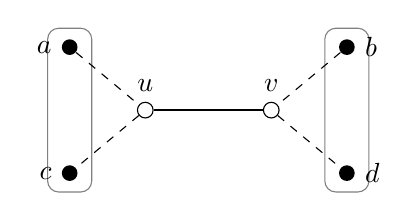
\begin{tikzpicture}[scale=.8]
 \draw[rounded corners,gray](-.35,-1.3) rectangle(.35,1.3);
 \draw[rounded corners,gray](4.05,-1.3) rectangle(4.75,1.3);
 \node[circle,fill=black,inner sep=2pt,label=left:$a$] (a) at(0,1){};
 \node[circle,fill=black,inner sep=2pt,label=left:$c$] (c) at(0,-1){};
 \node[circle,fill=black,inner sep=2pt,label=right:$b$] (b) at(4.4,1){};
 \node[circle,fill=black,inner sep=2pt,label=right:$d$] (d) at(4.4,-1){};
 \node[circle,draw,inner sep=2pt,label=above:$u$] (u) at(1.2,0){};
 \node[circle,draw,inner sep=2pt,label=above:$v$] (v) at(3.2,0){};
 \draw[dashed](a)--(u)--(c); \draw[dashed](b)--(v)--(d);
 \draw[thick](u)--(v);
\end{tikzpicture}
\caption{The common six-root configuration after the short-corner
exclusions. The boxes are the two positive opposite-pair blocks to
eliminate; their internal products are suppressed. Dashed lines show
allowed white contacts, with a nonempty subset chosen on each side.
The only cross connection is the nonright bridge $uv$; all omitted
cross contacts are zero.}
\label{fig:two-white-Schur}
\end{figure}

\begin{proposition}[The distinguished-bond argument]\label{prop:highfield}
A compact arithmetic21-polytope cannot have an actual ground field
$K$ which is not isomorphic to a subfield of $F$ and does not contain
$K_7$.
\end{proposition}
\begin{proof}
A Lann\'er diagram of order at least four has no bond of label
at least six: a neighboring nonright bond would give a proper
three-node determinant at most $1-3/4-1/4=0$. Dotted or parallel
bonds already fail a proper two-node test. All remaining entries
belong to $F$, contrary to Lemma~\ref{lem:detfield}. The same field
argument excludes triangles with all labels at most five. Label7
is impossible since its two-cycle generates $K_7$. Every remaining
triangle consequently has either a bond of label at least nine,
or a label6 or8 with both other bonds nonright. In the latter case
a right triangle would again have determinant in $F$.

Call such a bond distinguished. In any finite diagram it is an
entire rank-two component: a further nonright contact violates the
three-node positive-definiteness test above. In the quadrilateral
configuration just described, the white bridge therefore forces both
distinguished bonds onto the opposite black pairs.
If $c$ is their positive contact magnitude and $p,q$ are the
nonnegative white contact magnitudes, the projection cost is
\[
 C=\frac{p^2+q^2+2cpq}{1-c^2}.
\]
For label at least nine, one nonright contact gives $C>2$:
$\cos^2(\pi/9)>7/8$. To verify this strict bound, put
$z=2\cos(2\pi/9)>1$. The polynomial $z^3-3z+1$ is increasing
for $z>1$ and is $-1/8$ at $3/2$, so $z>3/2$.
For a distinguished label6 or8, both contacts are nonright and
$C\ge1/[2(1-c)]>2$, since $c\ge\sqrt3/2>3/4$.
The common obstruction proves a short marked corner on every quadrilateral.

Give one unit to distance-at-most-two marked pairs and one additional
unit to an entire $I_2(m)$ pair with $m\ge6$. A triangular face has
a minimal indefinite block containing all three black nodes: deleting
one leaves a finite corner. The full star has a negative direction,
as projection off its white support gives the normals bounding its
actual compact hyperbolic triangle. The minimal block is therefore
exactly that black triangle. Its two nonright bonds give payment
at least two. Quadrilaterals pay at least one as proved above.
For a connected finite tree the distance-two pair count is
\[
 (r-1)+\sum_v\binom{\deg v}{2}.
\]
It is $2r-3$ on a nontrivial path and $2r-2$ on a $D/E$ tree;
$A_1$ costs zero. The additional dihedral unit gives cost two,
also $2r-2$. Every rank21 forest thus costs at most40.
Lemma~\ref{lem:threshold} gives the contradiction.
\end{proof}

\subsection{The exact biquadratic field}
Assume now that the actual ground field is $F$, not a proper subfield.
The published arithmetic Lann\'er classification in
\cite[Section3.1, Figure1 and formula(4)]{Nikulin} puts the ground
fields of orders four and five in $\{\Q,\Q(\sqrt2),\Q(\sqrt5)\}$.
Lemma~\ref{lem:detfield} excludes those orders here. Order two remains
the full, unsampled family
\[
 \tau\in\mathcal O_F,\quad \Q(\tau)=F,\quad
 \tau>4,\quad 0<\sigma(\tau)<4\quad(\sigma\ne\mathrm{id}),
\]
with unit-normal product $-\sqrt\tau/2$. The preceding quadrilateral
argument eliminates an order-two minimal piece before using a triangle
list, so no bounded dotted-parameter search is needed in this field.

Put $t_m=2\cos(\pi/m)$ and $d_m=t_m^2$.
The condition $d_m\in F$ makes $\varphi(m)$ divide eight for $m\ge3$.
Every prime divisor of $m$ is2,3 or5, with exponents at most4,1,1.
Testing those finitely many products gives
\[
 2,3,4,5,6,8,10,12,15,16,20,24,30.
\]
Labels12 and24 contain $\Q(\sqrt3)$, not a subfield of $F$.
The real cyclotomic fields for15,16,20,30 are cyclic quartic:
the respective classes2,3,3,7 have order four in the unit group
modulo sign. They cannot equal the biquadratic field $F$.
The complete finite alphabet is therefore
\[
 \mathcal L=\{2,3,4,5,6,8,10\},\qquad
 (d_m)_{m\in\mathcal L}=(0,1,2,\phi^2,3,2+\sqrt2,2+\phi),
 \quad\phi=(1+\sqrt5)/2.
\]

\begin{certificate}[The finite triangle calculation]\label{cert:F25}
Among the $\binom{9}{3}=84$ unordered triples with repetition from $\mathcal L$,
the complete arithmetic Lann\'er triangles with actual field $F$ are
$(2,5,8)$ and $(4,5,5)$. The successive tests give:
\begin{center}\small
\begin{tabular}{lr}\toprule
First failed test or surviving class&Number\\\midrule
Not a compact hyperbolic triangle&13\\
Length-three cyclic product outside $F$&37\\
Proper ground subfield&28\\
Nonpositive conjugate determinant&4\\
All tests passed&2\\\bottomrule
\end{tabular}
\end{center}
\end{certificate}
Here is a complete exact algorithm for this finite proposition.
Enumerate $l\le m\le n$ from $\mathcal L$, reject reciprocal sum
at least one, and seek the nonnegative element
$P=\sqrt{d_ld_md_n}$ in $F$. Arithmetic is rational in the basis
$1,\sqrt2,\sqrt5,\sqrt{10}$; no floating sign decision occurs.
For completeness, square-root membership in a quadratic extension
$L(\sqrt d)$ reduces to square-root membership in $L$. To square
$y+z\sqrt d$ to $a+b\sqrt d$, solve
\[
 y^2+dz^2=a,\qquad 2yz=b.
\]
If $b=0$, test both $a$ and $a/d$ for squares in $L$.
If $b\ne0$, enumerate both possible roots
$r^2=a^2-db^2$ in $L$, test $y^2=(a+r)/2$ with $y\ne0$,
and put $z=b/(2y)$, verifying the square. Conversely every root
has exactly this form, so the test is complete. Apply it first to
$F=\Q(\sqrt2)(\sqrt5)$ and then to $\Q(\sqrt2)$; at the rational
base, numerator and denominator must be nonnegative integer squares.
The tower has fixed depth and every branch is finite.

For each successful $P$, the square-two determinant is
\[
 \Delta=2(4-d_l-d_m-d_n-P).
\]
Test the four sign changes of $\sqrt2,\sqrt5$ on the generators
$d_l,d_m,d_n,P$. Their common stabilizer is trivial precisely when
they generate $F$, by Galois correspondence. Finally require
$\sigma(\Delta)>0$ at the other three embeddings. Exact signs in
each quadratic tower follow by separating equal-sign summands or
squaring opposite-sign summands; for example
$\operatorname{sgn}(A+B\sqrt d)=\operatorname{sgn}(A)
\operatorname{sgn}(A^2-dB^2)$ when $A,B$ have opposite signs.
All cyclic products tested are integral because they are products of
algebraic integers $2\cos(\pi/m)$. Proper two-node minors are positive
at every embedding. These tests are consequently the arithmetic Gram
criterion for these triangles. The fixed loops terminate, cover every
triple, and return exactly the displayed partition and two survivors.
The standalone rational implementation and its saved exact records are
\path{scripts/fresh_sqrt2sqrt5_lanner_catalogue_20261016.py} and
\path{results/fresh_sqrt2sqrt5_lanner_catalogue_20261016.json}.

\begin{proposition}\label{prop:F25}
There is no compact arithmetic21-polytope with actual ground field $F$.
\end{proposition}
\begin{proof}
In the two-white quadrilateral configuration, a triangle whose opposite
black bond has label $m$ and white contacts $p,q$ has projection cost
\[
 C(m;p,q)=\frac{d_p+d_q+P}{4-d_m}.
\]
The five possible positions from Certificate~\ref{cert:F25} give
\begin{center}\small
\begin{tabular}{lll}\toprule
Triangle&Opposite bond&Cost\\\midrule
$(2,5,8)$&2&$(7+2\sqrt2+\sqrt5)/8$\\
$(2,5,8)$&5&$1+\sqrt2/2+\sqrt5/5+\sqrt{10}/10$\\
$(2,5,8)$&8&$3/2+3\sqrt2/4+\sqrt5/2+\sqrt{10}/4$\\
$(4,5,5)$&4&$3/2+3\sqrt2/4+\sqrt5/2+\sqrt{10}/4$\\
$(4,5,5)$&5&$2+\sqrt2+3\sqrt5/5+2\sqrt{10}/5$\\\bottomrule
\end{tabular}
\end{center}
The last four costs are greater than two. For the second row use
$\sqrt2>7/5$, $\sqrt5>2$ and $\sqrt{10}>3$, giving
$1+7/10+2/5+3/10=12/5>2$ strictly; the remaining rows already exceed two
from their first positive terms using $\sqrt2>1,\sqrt5>2$.
The first
position cannot occur: its white root meets a label8 bond and the
required nonright white bridge in a finite corner, whose three-node
determinant is at most $1-\cos^2(\pi/8)-1/4<0$.
The common Schur obstruction now proves a short corner on every
quadrilateral, with arbitrary other supporting whites retained.
Use only the distance-two base weights. Each of the two possible
black triangles has at least two nonright bonds, and so pays at least
two. The same tree count bounds every rank21 vertex by40, again
contradicting Lemma~\ref{lem:threshold}.
\end{proof}

\section{The thirteen fields and final composition}\label{sec:fields}
Let $K_m=\Q(\cos(2\pi/m))$. The dimension-at-least14 field restriction
\cite{Vinberg,Nikulin}
and the inherited complete field proofs give the following dimension 21
branches. The shorter list valid only from 22 is not used at21.
\begin{center}
\begin{tabular}{ll}\toprule
Actual field&Dimension21 exclusion\\\midrule
$\Q$&Simplest-type arithmeticity and Meyer isotropy\\
$\Q(\sqrt2)$&Complete all-white bound20 proof\\
$K_7$&Complete cubic-seven bound20 proof\\
$\Q(\sqrt3),\Q(\sqrt6),\Q(\sqrt2,\sqrt3)$&Proposition~\ref{prop:highfield}\\
$K_9,K_{11},K_{15},K_{16},K_{20}$&Same proposition, field checks below\\
$\Q(\sqrt2,\sqrt5)$&Proposition~\ref{prop:F25}\\
$\Q(\sqrt5)$&Proposition~\ref{prop:golden}\\\bottomrule
\end{tabular}
\end{center}
Here are the precise internal theorem interfaces behind
Proposition~\ref{prop:inherited}. The all-white $\Q(\sqrt2)$ theorem
excludes dimension21 using its complete arbitrary-white quadrilateral
closure and strict weight comparison; both parts are required, not
just the saved weight vector. Their common TeX exposition, including
the all-size attachments, is Section4 of the preserved technical
supplement \path{manuscripts/compact_arithmetic21.tex}. The supporting
exact proof reports are
\path{results/fresh_sqrt2_quad_exhaustion_20261015_review.md} and
\path{results/fresh_sqrt2_weight_bound_20261015_review.md}.
The cubic-seven bound20 theorem is the complete simultaneous-star rank
proof in \path{results/fresh_compact_global_bound_20261015.md}.

For the eight branches of Proposition~\ref{prop:highfield}, the only
subfields of $F$ are $\Q$, $\Q(\sqrt2)$, $\Q(\sqrt5)$,
$\Q(\sqrt{10})$ and $F$.
The three displayed square-root fields are not among them.
$K_9,K_{11}$ have degrees three and five; $K_{15},K_{16},K_{20}$
are cyclic quartic rather than biquadratic. None embeds in $F$.
All eight have degree indivisible by three, except $K_9$.
The cyclotomic fields of coprime conductors7 and9 have product
degree $\varphi(63)=\varphi(7)\varphi(9)$, so their intersection
is rational and $K_9$ does not contain $K_7$ either. This checks
both field hypotheses for every branch. Proposition~\ref{prop:F25}
uses exact field equality and is not applied to the golden proper subfield.

The original supporting derivations and exact records remain preserved
as \path{results/fresh_arithmetic_high_label_20261016.md} and
\path{results/fresh_sqrt2sqrt5_lanner_catalogue_20261016.md};
their geometric arguments have now been given here.
The rational branch uses simplest-type arithmeticity and Meyer:
the rational indefinite form in this rank is isotropic, so its
arithmetic quotient cannot be compact.

For dimensions22 through29, the published higher-dimensional field
restriction leaves $\Q(\sqrt2)$, $\Q(\sqrt5)$, $K_7$. The first and third
have the bound20 just stated; the golden bound21 uses the complete
native face domains and shared H3-hub rule in\newline
\path{results/fresh_sqrt5_h3_hub_coverage_20261016.md}.
The strict dimension-dependent $h$-vector threshold and the full forest
recurrence exclude each of these finitely many field/dimension branches.
Together with the published compact29 theorem this proves the first
assertion of Proposition~\ref{prop:inherited}. The thirteen dimension21
branches above prove its second assertion, without applying the
dimension22 field restriction at dimension21.
The preserved composition proofs are\newline
\path{results/fresh_compact21_single_field_20261016.md} and the
technical supplement cited in the introduction. Their binders check
dependency and branch coverage; they do not replace these component
theorems or reprove them by hashing their certificates.

\begin{proof}[Proof of Theorem~\ref{thm:main}]
Proposition~\ref{prop:inherited} excludes every dimension at least22.
At dimension21 its thirteen-branch reduction leaves only the golden
field. Proposition~\ref{prop:golden} excludes that field as
well. Hence every compact arithmetic chamber has dimension at most 20.
\end{proof}

\section{Reproducibility and verification boundaries}
The proof's finite objects are exact field/signature domains, literal
contact maps, finite-diagram orbit coefficients, native face payments
and forest maxima. Their explicit source and data pins are carried by
the rational reconstruction certificate. Reproduction needs no optimizer:
\begin{verbatim}
python3 -B \
  scripts/fresh_compact21_self_hub_exact40_reconstruction_20261018.py \
  --verify
python3 -B \
  scripts/check_compact21_self_hub_primal_independent_20261018.py \
  --candidate \
  results/fresh_compact21_self_hub_exact40_reconstruction_20261018.json
\end{verbatim}
Run these as separate sequential batches through
\path{scripts/run_bounded_research_check_20261018.py}, whose live watchdog
adds the 59-second cap,1GiB process-tree RSS limit and disk/RAM gates.
Each checker owns the shared exclusive lock. The first
reconstructs the saved candidate and checks every enlarged face and forest;
the second uses a separate implementation. Large inherited queue replays
are documented in the bound21 proof map and must also be scheduled in
bounded sequential batches. New final composition/hash checks bind their
existing certificates; they do not freshly regenerate those classifications.

The remaining validation boundaries must be explicit. Published
structural theorems may be assumptions in a formal interface. Internal
whole-star coverage, incidence priority arguments and exact certificate
logic must be formalized rather than silently imported as published
axioms. A Lean theorem assuming all field bounds would certify only the
last composition. The current result is an internally reviewed
computer-assisted proof with rational scripts and an independent
saved-primal evaluation; complete geometric Lean verification and
external review are separate tasks. No new high-dimensional chamber or
sharpness assertion follows.

\appendix
\section{Exact finite data and proof supplements}
The finite classifications in this paper use attached exact records,
with the mathematical domains and rejection tests stated above.
Their relevant proof and checker families are as follows. The listed
stems identify JSON data under \texttt{results/} and solver-free checkers
under \texttt{scripts/}. Written reports or separately named reviews
provide the accompanying proofs and replay records. In particular,
the triangle-coupling proof is in
\path{results/review_compact21_d5_two_e8_triangle_coupling_20261018.md}.
Full immutable dependency records remain in
the reproduction guide rather than being printed as hash lists here.
\begin{itemize}
\item The complete Lann\'er and 76-marking inputs are
\path{fresh_sqrt5_lanner_catalogue_20261015} and
\path{fresh_sqrt5_triangle_weights_20261015}. A marking record has
the literal graph labels, three black nodes, complementary white set,
three finite corner graphs and their exact payments. The first
catalogue has its separate exact arithmetic and topology replay.
\item The initial union and 24 Schur families are
\path{fresh_sqrt5_quad_exhaustion_20261015} and
\path{fresh_sqrt5_dotted_parameters_20261015}. Their schema and
bounded field domains are those in Proposition~\ref{prop:domains}.
The finite and dotted queues, their singular stopping obligations and
literal marked maps are independently evaluated in the two queue
review reports cited after Proposition~\ref{prop:coverage}.
\item The active D5 proof uses
\path{fresh_compact21_d5_fork_quad_triangle_priority_20261018},
its Lambert and one-basic-unit reports, and
\path{fresh_compact21_d5_mixed_fork_quad_exclusion_20261018}.
The checker domains are the 25 ordered pairs of the five finite
endpoint types and the exact Schur polynomials and field obstructions
displayed above, not a bounded distance search.
\item The full inactive consumer is
\path{fresh_compact21_extreme_e8_quad_consumer_completeness_20261018}.
Its records retain the entire finite D5 two-root attachment domain,
both orientations, short unit intervals and exact coefficient identities.
The preliminary triangle types come from
\path{fresh_compact21_d5_two_e8_triangle_coupling_20261018} and its
separate written review; each root record has its full contact vector,
height, two positive corner tests and conjugate field test.
\item The 1024-vector H4 domain and four deficient rows are
\path{fresh_compact21_h4_a1_triangle_priority_20261018}.
Each eligible row records the five native contacts, exact height,
cycle tests and all three modified triangle payments. The strengthened
source capacity is
\path{fresh_compact21_a5_h4_source_capacity_20261018}; its entire
calculation is the two endpoint inverse entries and positive forced
product given in the text.
\end{itemize}
The accompanying reports identify the finite domains and their exact
execution records. The inherited field theorems remain the explicit companion
interfaces of Proposition~\ref{prop:inherited}, with their technical
proof homes in Section~\ref{sec:fields}.

\begin{thebibliography}{9}
\bibitem{Vinberg} E. B. Vinberg, \emph{Absence of crystallographic groups
of reflections in Lobachevskii spaces of large dimension}, Transactions
of the Moscow Mathematical Society47 (1984),75--112. Original text:
\url{https://www.mathnet.ru/php/getFT.phtml?jrnid=mmo&option_lang=rus&paperid=444&what=fullt}.
\bibitem{Nikulin} V. V. Nikulin, \emph{On ground fields of arithmetic
hyperbolic reflection groups}, Introduction and Sections2,3,
\url{https://arxiv.org/abs/0708.3991}.
\bibitem{Belolipetsky} M. Belolipetsky, \emph{Arithmetic hyperbolic
reflection groups}, Lemma2.1 and Sections1,7,
\url{https://arxiv.org/abs/1506.03111}.
\bibitem{Internal} Exact internal sources, geometric reviews and immutable
certificate interfaces, listed in
\path{results/compact_arithmetic20_universal_composition_20261018.md},
\path{results/fresh_compact21_self_hub_exact40_reconstruction_20261018.md},
and \path{docs/compact_arithmetic21_proof_map.md}.
\end{thebibliography}
\end{document}
